\section{Results \& Discussion}
Figures~\ref{fig:dspcccref}, and \ref{fig:dspcmartref} compare the reflectometry and SLD profiles from each of the different methods at each surface pressure.
It is clear that the trends for all datasets are simulation.
In addition, the $\chi^2$ between each of the models and the experimental data for each contrast at an APM associated with a surface pressure of \SI{30}{\milli\newton\per\meter}, the average $\chi^2$ and standard deviation for each method are given in Table~\ref{tab:chi}.
%
\begin{figure}
    \centering
    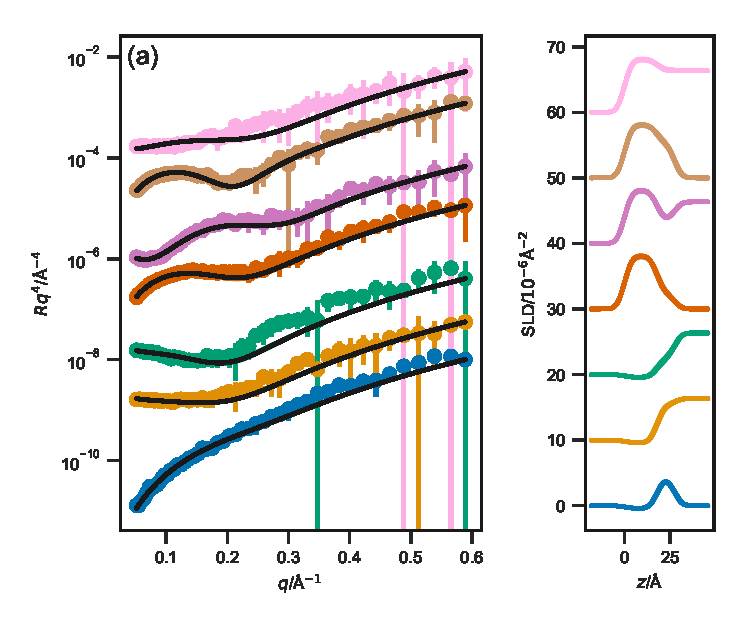
\includegraphics[width=0.49\textwidth]{reflectometry2/dspc_20_ref_sld}
    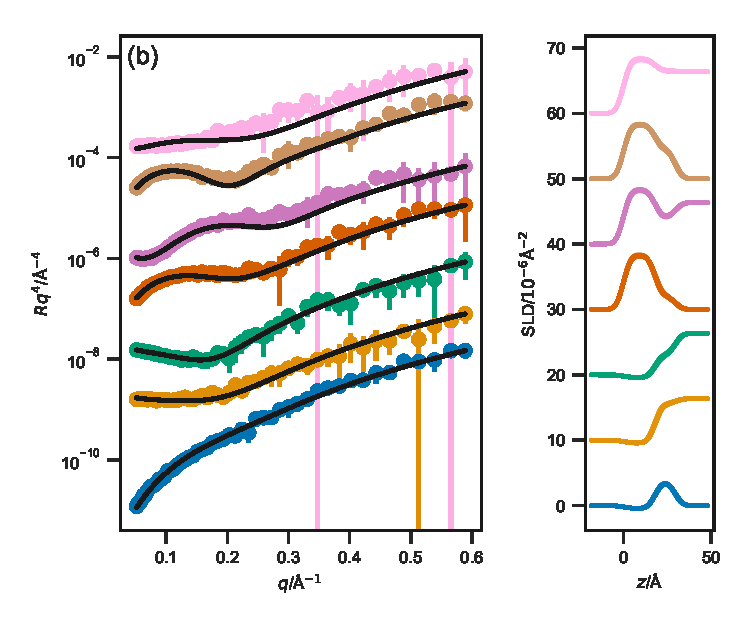
\includegraphics[width=0.49\textwidth]{reflectometry2/dspc_30_ref_sld}\\
    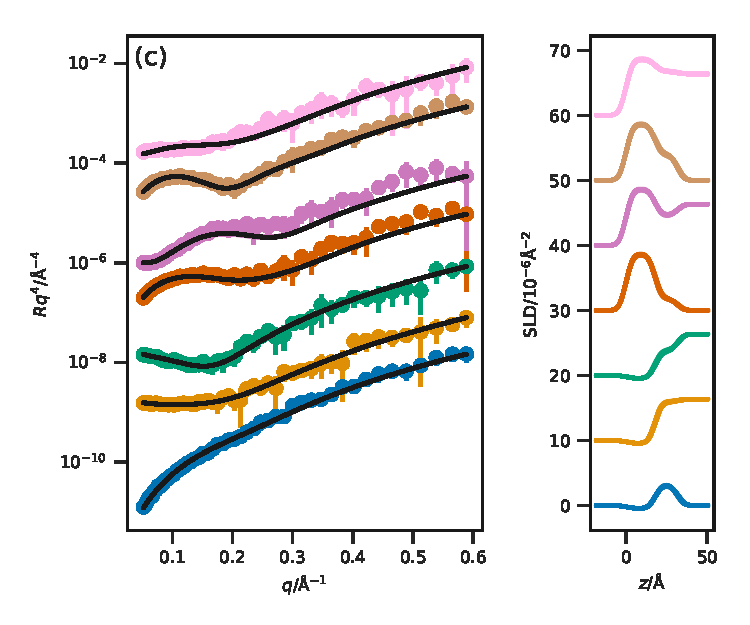
\includegraphics[width=0.49\textwidth]{reflectometry2/dspc_40_ref_sld}
    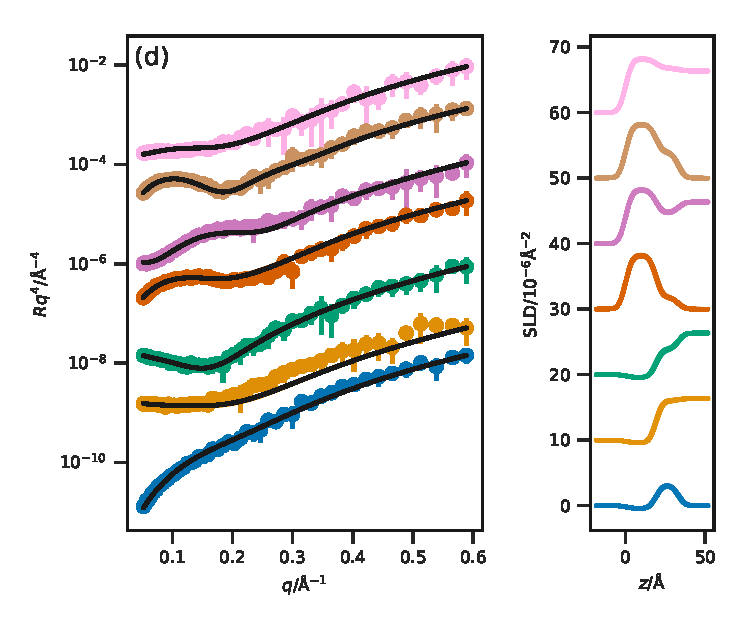
\includegraphics[width=0.49\textwidth]{reflectometry2/dspc_50_ref_sld}
    \caption{The NR profiles (left) and SLD profiles (right) determined from the chemically-consistent model for DSPC; (a) at \SI{20}{\milli\newton\per\meter}, (b) at \SI{30}{\milli\newton\per\meter}, (c) at \SI{40}{\milli\newton\per\meter}, and (d) at \SI{50}{\milli\newton\per\meter}. From top-to-bottom the contrasts are as follows; d${_83}$-\ce{D2O}, d${_83}$-ACMW, d${_70}$-\ce{D2O}, d${_70}$-ACMW, h-\ce{D2O}, d${_13}$-\ce{D2O}, d${_13}$-ACMW. The different contrast NR profiles have been offset in the \emph{y}-axis by an order of magnitude and the SLD profiles offset in the \emph{y}-axis by \SI{10e-6}{\per\angstrom\squared}, for clarity.}
    \label{fig:dspcccref}
\end{figure}
%
%
\begin{figure}
    \centering
    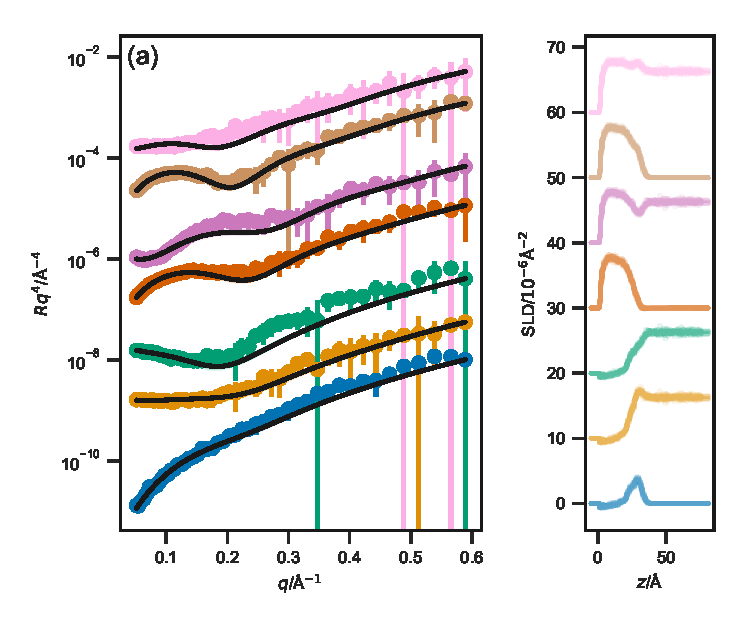
\includegraphics[width=0.49\textwidth]{reflectometry2/dspc_slipids_20_ref_sld}
    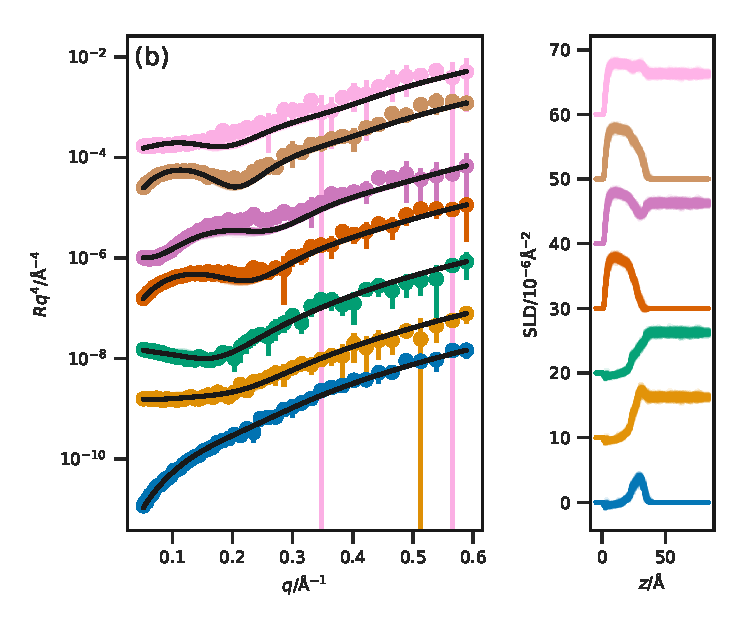
\includegraphics[width=0.49\textwidth]{reflectometry2/dspc_slipids_30_ref_sld}\\
    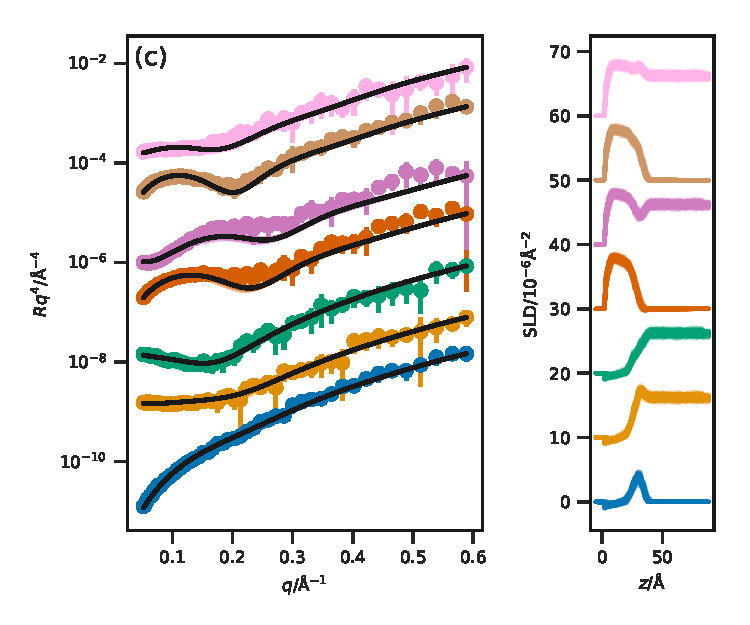
\includegraphics[width=0.49\textwidth]{reflectometry2/dspc_slipids_40_ref_sld}
    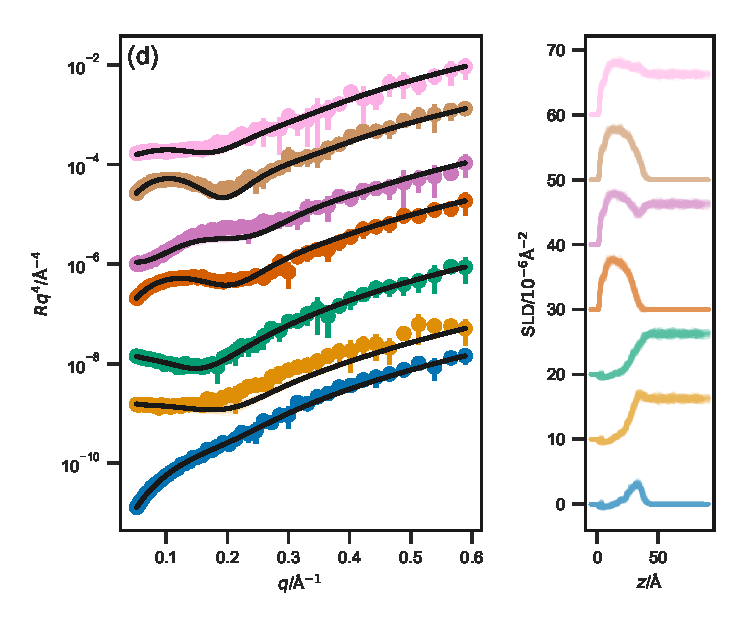
\includegraphics[width=0.49\textwidth]{reflectometry2/dspc_slipids_50_ref_sld}
    \caption{The NR profiles (left) and SLD profiles (right) determined from the Slipid all-atom potential model simulations of DSPC; (a) at \SI{20}{\milli\newton\per\meter}, (b) at \SI{30}{\milli\newton\per\meter}, (c) at \SI{40}{\milli\newton\per\meter}, and (d) at \SI{50}{\milli\newton\per\meter}. From top-to-bottom the contrasts are as follows; d${_83}$-\ce{D2O}, d${_83}$-ACMW, d${_70}$-\ce{D2O}, d${_70}$-ACMW, h-\ce{D2O}, d${_13}$-\ce{D2O}, d${_13}$-ACMW. The different contrast NR profiles have been offset in the \emph{y}-axis by an order of magnitude and the SLD profiles offset in the \emph{y}-axis by \SI{10e-6}{\per\angstrom\squared}, for clarity.}
    \label{fig:dspcmartref}
\end{figure}
%
%
\begin{figure}
    \centering
    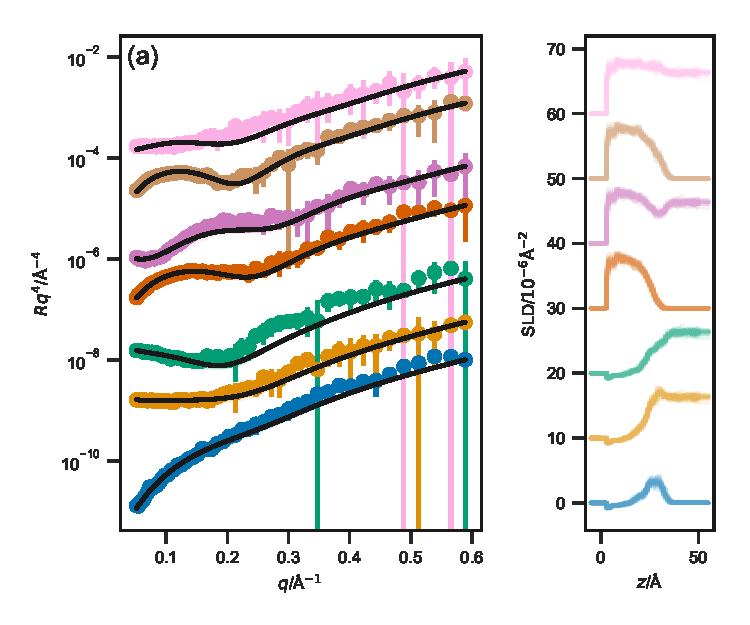
\includegraphics[width=0.49\textwidth]{reflectometry2/dspc_berger_20_ref_sld}
    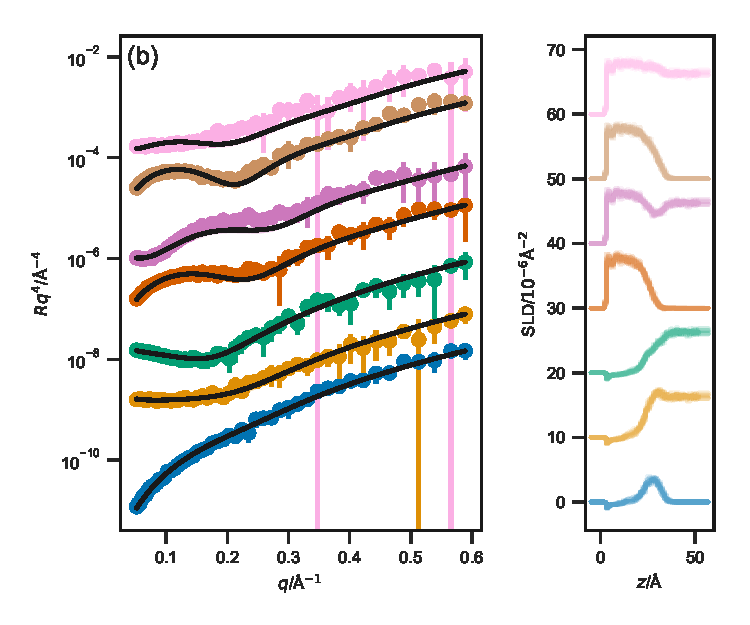
\includegraphics[width=0.49\textwidth]{reflectometry2/dspc_berger_30_ref_sld}\\
    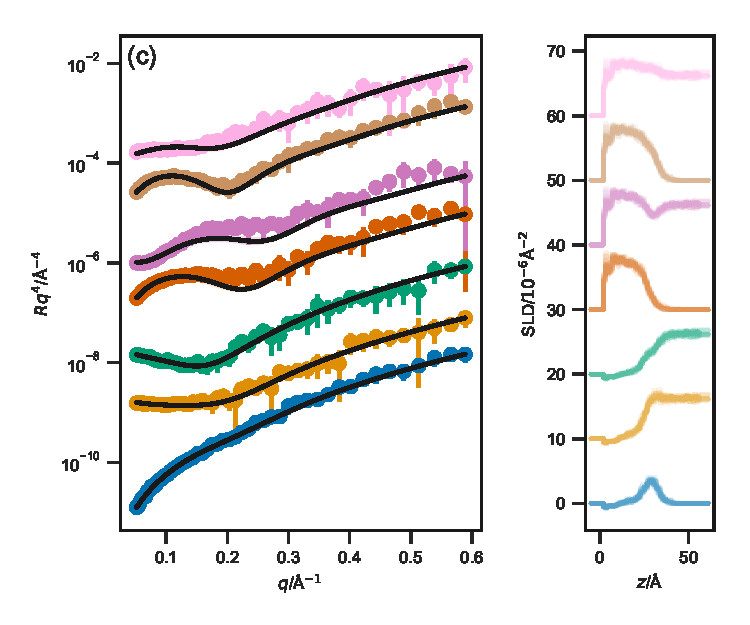
\includegraphics[width=0.49\textwidth]{reflectometry2/dspc_berger_40_ref_sld}
    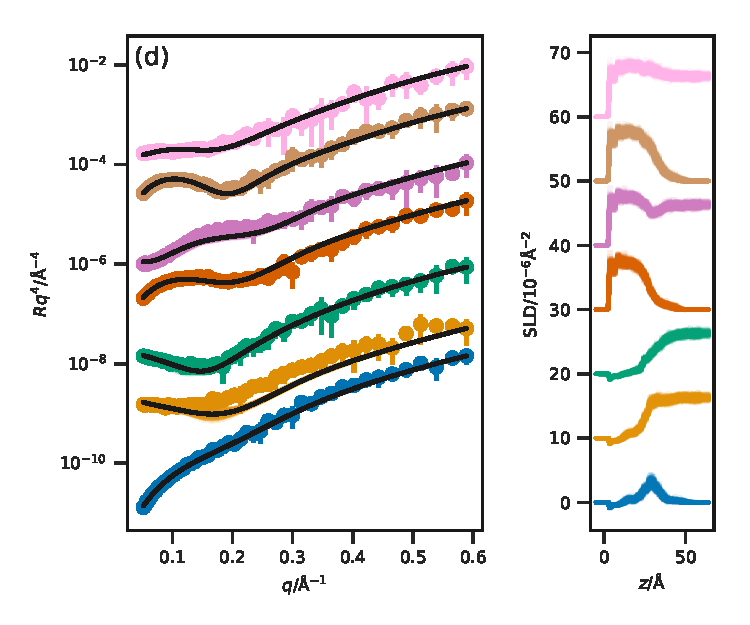
\includegraphics[width=0.49\textwidth]{reflectometry2/dspc_berger_50_ref_sld}
    \caption{The NR profiles (left) and SLD profiles (right) determined from the Berger united-atom potential model simulations of DSPC; (a) at \SI{20}{\milli\newton\per\meter}, (b) at \SI{30}{\milli\newton\per\meter}, (c) at \SI{40}{\milli\newton\per\meter}, and (d) at \SI{50}{\milli\newton\per\meter}. From top-to-bottom the contrasts are as follows; d${_83}$-\ce{D2O}, d${_83}$-ACMW, d${_70}$-\ce{D2O}, d${_70}$-ACMW, h-\ce{D2O}, d${_13}$-\ce{D2O}, d${_13}$-ACMW. The different contrast NR profiles have been offset in the \emph{y}-axis by an order of magnitude and the SLD profiles offset in the \emph{y}-axis by \SI{10e-6}{\per\angstrom\squared}, for clarity.}
    \label{fig:dspcmartref}
\end{figure}
%
%
\begin{figure}
    \centering
    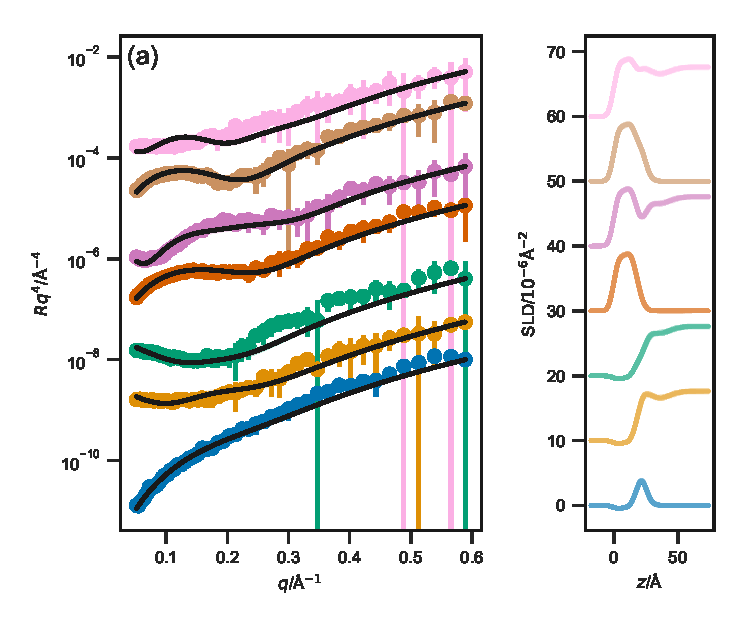
\includegraphics[width=0.49\textwidth]{reflectometry2/dspc_martini_20_ref_sld}
    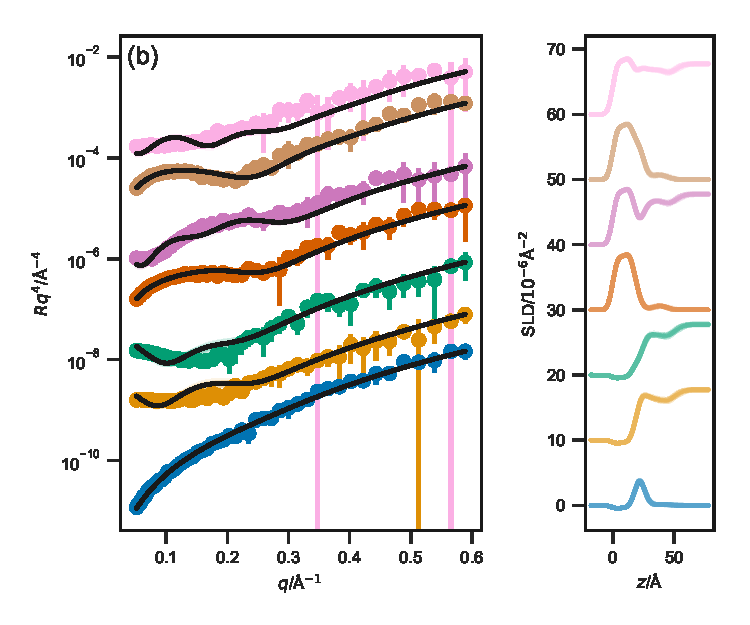
\includegraphics[width=0.49\textwidth]{reflectometry2/dspc_martini_30_ref_sld}\\
    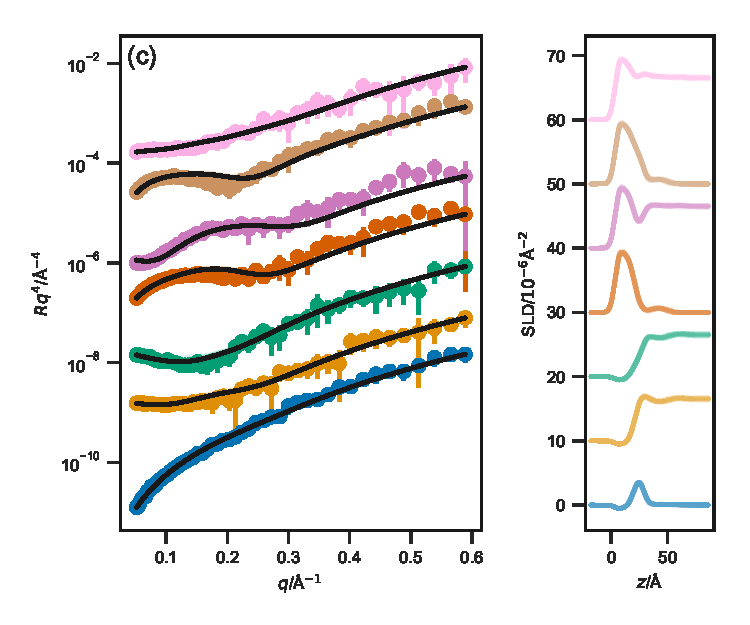
\includegraphics[width=0.49\textwidth]{reflectometry2/dspc_martini_40_ref_sld}
    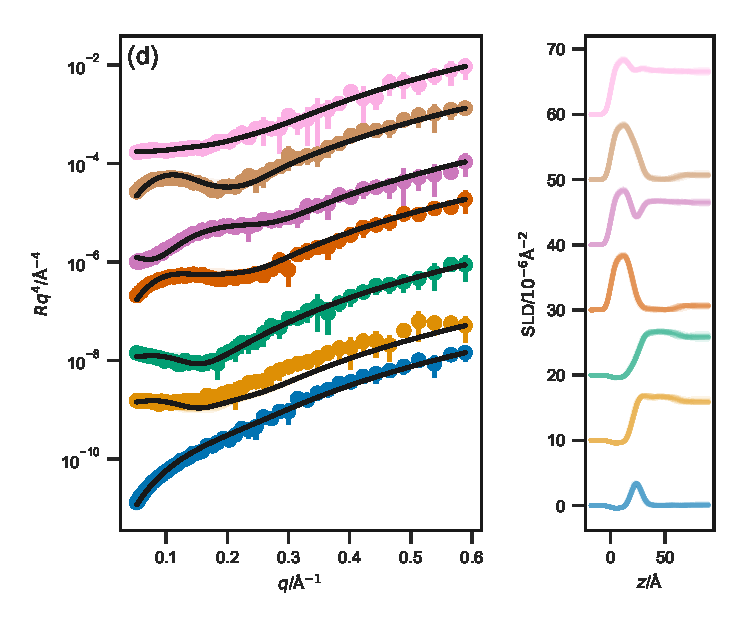
\includegraphics[width=0.49\textwidth]{reflectometry2/dspc_martini_50_ref_sld}
    \caption{The NR profiles (left) and SLD profiles (right) determined from the MARTINI coarse-grained potential model simulations of DSPC; (a) at \SI{20}{\milli\newton\per\meter}, (b) at \SI{30}{\milli\newton\per\meter}, (c) at \SI{40}{\milli\newton\per\meter}, and (d) at \SI{50}{\milli\newton\per\meter}. From top-to-bottom the contrasts are as follows; d${_83}$-\ce{D2O}, d${_83}$-ACMW, d${_70}$-\ce{D2O}, d${_70}$-ACMW, h-\ce{D2O}, d${_13}$-\ce{D2O}, d${_13}$-ACMW. The different contrast NR profiles have been offset in the \emph{y}-axis by an order of magnitude and the SLD profiles offset in the \emph{y}-axis by \SI{10e-6}{\per\angstrom\squared}, for clarity.}
    \label{fig:dspcmartref}
\end{figure}
%
%
\begin{table}
    \centering
    \small
    \caption{The $\chi^2$ values for each of the reflectometry model at an APM associated with a surface pressure of \SI{30}{\milli\newton\per\meter}.}
    \label{tab:chi}
    \begin{tabular}{l | l l l l}
        \toprule
        Contrast & Chemically-consistent & Slipids & Berger & MARTINI \\
        \midrule
        h-\ce{D2O} & \input{output/reflectometry2/dspc_30/dspc_30_hd2o_chi.txt} & \input{output/reflectometry2/dspc_30/dspc_slipids_30_hd2o_chi.txt} & \input{output/reflectometry2/dspc_30/dspc_berger_30_hd2o_chi.txt} & \input{output/reflectometry2/dspc_30/dspc_martini_30_hd2o_chi.txt} \\
        d$_{13}$-\ce{D2O} & \input{output/reflectometry2/dspc_30/dspc_30_d13d2o_chi.txt} & \input{output/reflectometry2/dspc_30/dspc_slipids_30_d13d2o_chi.txt} & \input{output/reflectometry2/dspc_30/dspc_berger_30_d13d2o_chi.txt} & \input{output/reflectometry2/dspc_30/dspc_martini_30_d13d2o_chi.txt} \\
        d$_{13}$-ACMW & \input{output/reflectometry2/dspc_30/dspc_30_d13acmw_chi.txt} & \input{output/reflectometry2/dspc_30/dspc_slipids_30_d13acmw_chi.txt} & \input{output/reflectometry2/dspc_30/dspc_berger_30_d13acmw_chi.txt} & \input{output/reflectometry2/dspc_30/dspc_martini_30_d13acmw_chi.txt} \\
        d$_{70}$-\ce{D2O} & \input{output/reflectometry2/dspc_30/dspc_30_d70d2o_chi.txt} & \input{output/reflectometry2/dspc_30/dspc_slipids_30_d70d2o_chi.txt} & \input{output/reflectometry2/dspc_30/dspc_berger_30_d70d2o_chi.txt} & \input{output/reflectometry2/dspc_30/dspc_martini_30_d70d2o_chi.txt} \\
        d$_{70}$-ACMW & \input{output/reflectometry2/dspc_30/dspc_30_d70acmw_chi.txt} & \input{output/reflectometry2/dspc_30/dspc_slipids_30_d70acmw_chi.txt} & \input{output/reflectometry2/dspc_30/dspc_berger_30_d70acmw_chi.txt} & \input{output/reflectometry2/dspc_30/dspc_martini_30_d70acmw_chi.txt} \\
        d$_{83}$-\ce{D2O} & \input{output/reflectometry2/dspc_30/dspc_30_d83d2o_chi.txt} & \input{output/reflectometry2/dspc_30/dspc_slipids_30_d83d2o_chi.txt} & \input{output/reflectometry2/dspc_30/dspc_berger_30_d83d2o_chi.txt} & \input{output/reflectometry2/dspc_30/dspc_martini_30_d83d2o_chi.txt} \\
        d$_{83}$-ACMW & \input{output/reflectometry2/dspc_30/dspc_30_d83acmw_chi.txt} & \input{output/reflectometry2/dspc_30/dspc_slipids_30_d83acmw_chi.txt} & \input{output/reflectometry2/dspc_30/dspc_berger_30_d83acmw_chi.txt} & \input{output/reflectometry2/dspc_30/dspc_martini_30_d83acmw_chi.txt} \\
        \midrule
        Average & \input{output/reflectometry2/dspc_30/dspc_30_all_chi.txt} & \input{output/reflectometry2/dspc_30/dspc_slipids_30_all_chi.txt} & \input{output/reflectometry2/dspc_30/dspc_berger_30_all_chi.txt} & \input{output/reflectometry2/dspc_30/dspc_martini_30_all_chi.txt} \\
        \bottomrule
    \end{tabular}
\end{table}
%

\subsection{MARTINI}
Initally, the MARTINI coarse-grained simulations were analysed with a layer thickness of \SI{1}{\angstrom} and an interfacial roughness of \SI{0}{\angstrom}, in a similar fashion to the other potential models.
However, as can be seen in Figure~\ref{fig:martorder} there is a clear ordering effect present in the MARTINI water, despite the use of the polarised water model.
The effect of this ordering on the SLD profile, and therefore the reflectometry profile, can be reduced by using a larger layer thickness and introducing an interfacial roughness.
Therefore, in the results disscussed below the MARTINI potential model simulation were analysed using a layer thickness of \SI{4}{\angstrom} and an interfacial roughness of \SI{0.2}{\angstrom}.
It is noted that this structuring may be reduced through the use of a less ordered wall \cite{koutsioubas_combined_2016} at the extreme of the simulation cell, however, the aim was to reproduce the experimental conditions using off-the-shelf tools and this would require custom modifications not easily available.
%
\begin{figure}
    \centering
    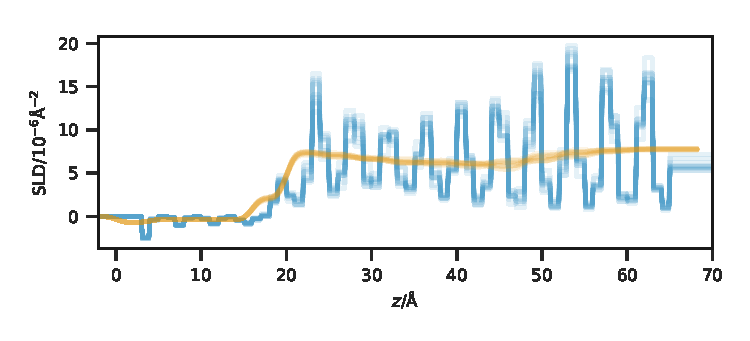
\includegraphics[width=0.80\textwidth]{reflectometry2/martini_order}
    \caption{A comparison of the scattering length density profile for the MARTINI potential model simulations at an APM associated with a surface pressure of \SI{30}{\milli\newton\per\meter}; the blue line shows the data where the layer thickness was \SI{1}{\angstrom} and no interfacial roughness and the orange line shows that with a layer thickness of \SI{4}{\angstrom} and a roughness of \SI{0.8}{\angstrom}}
    \label{fig:martorder}
\end{figure}
%

It can be seen from Table~\ref{tab:chi} that even with the larger layer thickness and adding interlayer roughness, the MARTINI potential model simulations do not effectively reproduce the reflectometry profile.
Furthermore, it is noted that the agreement with the contrasts containing \ce{D2O} is particularly poor, this is most likely an artefact of the structuring effect mentioned above which cannot be completely removed.

However, it is noted that the agreement for the samples where the contrast uses ACMW, where the water is effectively removed from the SLD profile is also poor.
This indicates that there are other artefacts limiting the applicability of the MARTINI potential model.
Another such artefact is clear from investigating the calculated calculated length of the hydrocarbon tail from the MARTINI simulation, at an APM associated with a surface pressure of \SI{30}{\milli\newton\per\meter}, which was found to be xxx, significantly less than the \SI{24.3}{\angstrom} estimated by the Tanford equation \cite{tanford_hydrophobic_1980}.
This is due to the nature of the MARTINI's 4-to-1 beading process, as DSPC has a hydrocarbon tail consisting of 18 carbon atoms, and it is not possible to bead such a chain accurately with the MARTINI potential model.
In this work, a MARTINI phospholipid molecules was used with 4 MARTINI beads making up the chain; corresponding to an all-atom hydrocarbon chain of 16 atoms.
Applying the Tanford equation to a hydrocarbon chain of such a length results in an anticipated length of \SI{18.7}{\angstrom}, which agress better with that found from simulation.

BLAHBLAH BIG WATER MOLECULES SOLVATE BADLY.

The requirement for a 4-to-1 beading strategy for the MARTINI potential model is a significant weakness.
A better method may be limiting experiments to system that can be modelled exactly or the use of a different beading model.
However, we are not aware of an off-the-shelf coarse-grained potential model that would easily offer the exact beading of DSPC.

\subsection{Comparison with other simulations}
Table~\ref{tab:chi} shows that both the Slipid and Berger potential model simulations agree well with the experimental data, with the Slipid potential model offering a slight improvement over the Berger.
The quality of agreement between these higher-resolution potential models and the chemically-consistent model is relatively similar.
However, the chemically-consistent model still offers a better fit to the experimental data than those determined from DM simulation.

The result that the chemically-consistent model offers better agreement with the data than those from even all-atom simulations is to be expected though, simply by considering the level of constraint present in implicity when determining the reflectometry profile directly from simulation.
While the chemically-consistent constrains the layer model to ensure that the number of phospholipid head groups is the same as the pairs of tail groups, those from MD simulation have more realistic chemical constraints present from the potential model; e.g. bonding of atoms, and the non-bonded potentials.
The quality of the agreement from this multi-moda approach is sufficient for such a method to be applied regularly to the analysis of neutron reflectometry.

Both the Slipid and Berger potential model simulations produced values for the tail length taht were in better agreement with that from the Tanford equation than the MARTINI potential model simulations.
For the Slipid potential model, with simulations at a APM associated with a surface pressure of \SI{30}{\milli\newton\per\meter} the tail length was found to be xx, while for the Berger potential model, at the same APM, a value of xx was obtained.
Neither is quite as large as the \SI{24.3}{\angstrom} from the Tanford equation, however, it should be noted that this value is considered a theoretical maximum for a fully extended carbon chain.

Using the molecular dynamics simulations and the chemically-consistent model, it is possible to compare the number of water molecules per head group.
From the Slipid and Berger potential model simulations, the number of water molecules per head group at an APM associated with a surface pressure of \SI{30}{\milli\newton\per\meter} was found to be xx and xx respectively.
These are in good agreement with the value of xx found from the chemically-consistent model, using Equation~\ref{equ:wph}.

It should be noted that to obtain the \SI{50}{\nano\second} production run simulation using the all-atom Slipid potential model required over 13 days of using 32 cores of the SCARF computing resource.
This is non-trivial and therefore not necessarily applicable to all neutron reflectometry measurements.
However, for the nearly as accurate Berger potential model simulations (which are only marginally less accurate), only approximately 2 day of the same compute resource was required.
This suggests that given the quality of agreement with the experimental data achieved from, and compute requirement for, the Berger potential model simulations, such simulations could be run alongside experiments at large facilities to aid interpretation and analysis.

\subsection{Using the Slipid potential model simulations to improve the monolayer model}
Despite the chemically-consistent model offering a small improvement in agreement over the Slipid potential model simulation, we believe that it is possible to use the MD simulations to improve the existing this model.
A possible improvement can be found from considering Figure~\ref{fig:nd}, which shows the water molecules per head gorup as a function of depth; it is clear that solvent penetration within the phospholipid head layer is not uniform.
In particular, there is a clear pocket of water formed around the ester group of the phospholipid.
However, currently the solvation is described as a uniform averaging of the head layer SLD profile with the SLD of the solvent.
The structuring in the solvation suggests that perhaps a different model for solvent penetration could be applied to the head layer to more accurately describe the realistic solvent penetration.

It is generally suggest that the conformal roughness between the layers should be carried evenly through the monolayer, when there is only a single phospholipid type \cite{campbell_structure_2018}.
However, from Figure~\ref{fig:nd}, it is clear that the overlap between the head layer and water is much larger than that between the tail and head.
Furthermore, there is additionally some solvent present deep within the tail layer, due to the presence of head group character within that region.
While the interfacial roughness can be considered as describing the capillary wave from the water surface, it is also frequently applied to account for the intrinsic/structure roughness in the monolayer that exists due to the fact that the phospholipid ensemble comprises of molecules with different conformations and thus different chain lengths.
This suggests that perhaps the constraint that the interfacial roughness should be constant through the monolayer might be relaxed.
